\documentclass[12pt]{article}

\usepackage[english]{babel}
\usepackage[utf8x]{inputenc}
\usepackage{mathtools}
\usepackage{graphicx}
\usepackage[colorinlistoftodos]{todonotes}

\begin{document}

\title{Fundamentals of Multivariable Calculus}
\author{Newlyn Joseph PhD}

\maketitle

\section{Introduction}

Multivariable calculus extends upon a traditonal single variable calculus course. It covers a broad spectrum opf topics, that essentially one up the topics typically taught in an introductory calculus course. This book does not touch upon every topic, but does highlight several important aspects of multivariable calculus that require mastery.

If you do not know any calculus basics, please put this book down. If you know what a Taylor polynomial is, you should be fine.

\subsection{The Extension}

As mentioned earlier, multivariable calculus extends upon the basic topics of single variable calculus. For example, the same principles utilized to find tangent lines to curves will be applied to finding tangent planes to three dimensional functions and surfaces.

\subsection{The Limitations}

Multivariable calculus, as the name implies, consists of functions of several variables. No longer are we confined to a traditional, two-dimensional Cartesian coordinate system. Throughout this text, we will explore several systems, ranging from polar coordinate systems to three dimensional systems, to even four dimensional systems (with color representing the fourth dimension).

As always, the only limitation we will ever run into is our minds. Keeping track of several variables and geometrically analyzing functions becomes a problem when we run out of dimensions. This is a typical issue that mathematicians are addressing.

\subsection{Course Objectives}

There are several objectives this course will address. They are as follows:

\begin{enumerate}
\item A Review of Partial Differentiation and Parametric Equations
\item Vectors, Component Notation, and Vector Operations
\item Dot Producs and their Applications
\item Integration, Differentiation, and Limits with Vectors
\item Gradient Vectors and their Properties
\item The Chain Rule for Paths
\dots
\end{enumerate}

I hope this book is of great use to any student who wants to review multivariable calculus concepts, or explore such concepts before undertaking a formal study.

\section{A Review of Partial Differentiation and Parametric Equations}

In this section, we will briefly review how to partially differentiate, and how to manipulate parametric equations.

\subsection{Partial Notation}

Typically, in calculus we see the term: $$\frac { dy }{ dx } $$
As we all know, this is read as "the derivative of y with respect to x".
This notation is very useful in single variable calculus, or functions of one variable. For example the function below could have its derivative represented beautifully with the notation descibed above: $$f(x) = x^2$$

This is however, not the best notation to descibe a more complex function, one which involves more than just two variables: $f(x,y) = x^2 + y^2$
For the function above, there are two derivatives we can obtain. They are as follows:$\frac { \partial z }{ \partial x } $ and $\frac { \partial z }{ \partial y } $ where $z$ is $f(x,y)$.

These notations are read as "partial z with respect to x" and "partial z with respect to y", respectively.

\subsection{Taking Partial Derivatives}

$$z = x^2 + y^2$$
Examine the function above. Notice how it is composed of three variables. Therefore, it would require a three dimensional coordinate system to visualize this geometrically. 

\begin{figure}[ht!]
\centering
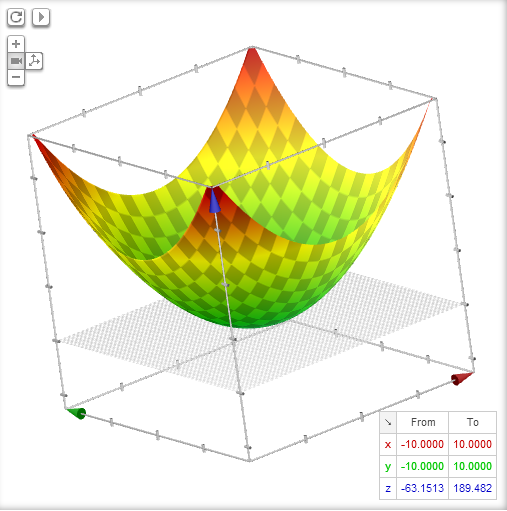
\includegraphics[width=90mm]{images/image.png}
\caption{$z = x^2 + y^2$}
\label{overflow}
\end{figure}

We can only differentiate with respect to one variable at a time. This essentially means that we can find how z changes with respect to x, and how z changes with respect to y. In order to take these derivatives we must ensure that the variable we aren't differentiating is held constant.

So, to find $\frac { \partial z }{ \partial x } $ let us hold y as a constant and differentiate with respect to x.

\begin{align}
\frac { d }{ dx }(z)\quad&=\quad\frac { d }{ dx } ({ x }^{ 2 }+{ y }^{ 2 }) \\
\frac { dz }{ dx }\quad&=\quad\frac { d }{ dx } ({ x }^{ 2 })+\frac { d }{ dx } ({ y }^{ 2 }) \\
\frac { dz }{ dx }\quad&=\quad2x\quad +\quad0 \\
\quad \quad \frac { dz }{ dx }\quad&=\quad2x
\end{align}

Notice how in step 3, we held the term with y as a constant, therefore it went to zero? That is the key step in partial differentiation: Hold all variables you are not respecting as constant! Similarly, we can differentiate z with respect to y, by holding x constant.

\begin{align}
\frac { d }{ dx }(z)\quad&=\quad\frac { d }{ dy } ({ x }^{ 2 }+{ y }^{ 2 }) \\
\frac { dz }{ dy }\quad&=\quad\frac { d }{ dy } ({ x }^{ 2 })+\frac { d }{ dy } ({ y }^{ 2 }) \\
\frac { dz }{ dy }\quad&=\quad0\quad +\quad2y \\
\quad \quad \frac { dz }{ dy }\quad&=\quad2y
\end{align}

So now you can take partial derivatives. Congratulations. Swag.

\subsection{Parametric Equations}

Parametric equations are literally just another style of writing a multivariable function. They are heavily used in physics, and an application of their use is in the plotting of a projectile's path.

A set of parametric equations utilizes a third variable, typically called $t$, that is typically used to represent time.

The following is an example:$$x = t^2 + t$$$$y  =2t - 1$$

Notice how plugging in a value of $t$ will provide you with an x value and a y value. It essentially provides you a coordinate.

You do not need to keep the equation of a curve in parametric form all the time. It is useful during some instances, but dring other instances, you want a function that directly relates x to y.

The set of parametric equations above can be easily written as a single equation by means of algebraic manipulation. We can elimate the parameter ($t$) through substitution.

\begin{align*}
y\quad&=\quad2t-1\\
y+1&=\quad2t\\
\frac{ 1 }{ 2 }(y+1)&=t
\end{align*}

The algebraic manipulation above rewrites one parametric equation in terms of $t$. This can be substituted into the second parametric equation.

This will yield the an equation solely in terms of x and y. This can be plotted.

\begin{align*}
x\quad=\quad \left( \frac { 1 }{ 2 } (y+1) \right) ^{ 2 }+\left( \frac { 1 }{ 2 } (y+1) \right) 
\end{align*}

\section{Vectors, Component Notation, and Vector Operations}

\subsection{vectors}


\end{document}
